%\documentclass[12pt]{article}
\documentclass[english]{sobraep}

\usepackage[utf8]{inputenc}
\usepackage[table]{xcolor}
\usepackage{geometry}
\geometry{a4paper, portrait, margin=2cm, top=2cm, bottom=2cm}
\usepackage{graphicx}
\usepackage[
  colorlinks=false,
  linkcolor=blue
]{hyperref}
\newcommand\rurl[1]{%
  \href{http://#1}{\nolinkurl{#1}}%
}
\usepackage{gensymb}
\usepackage{fancyvrb}
\usepackage{breqn}
\usepackage{times}
\usepackage{float}
\usepackage{svg}
\usepackage{tabularx}
\usepackage{lscape}
\usepackage{pdflscape}
\usepackage[
backend=biber,
style=numeric-comp,
sorting=none,
backref=true,
mincitenames=1,
maxcitenames=3,
maxbibnames=99
]{biblatex}
\usepackage{amsmath}
\usepackage{blindtext}
\usepackage{hyperref}
\usepackage{cuted}
\addbibresource{references.bib}% Syntax for version >= 1.2

\title{Review of Recent Advancements in RMIS Using dVRK\\(ROBOTICS M - TECHNICAL ESSAY)}



%\author{Ross J. Gardiner\\
%	\normalsize \textbf{Email}: 2190583g@student.gla.ac.uk\\
%	\normalsize \textbf{Matric. nr.}: 2190583g
%}


\begin{document}
\maketitle
\begin{tabular}{l|c}
 Author: & \textbf{Ross J. Gardiner}   \\
 Course code: & \verb|ENG5326| \\
 Matric nr: & \verb|2190583g| \\
Online: & \rurl{shorturl.at/bnpJY}   \\
\end{tabular}
%\begin{minipage}{0.4\linewidth}
%\begin{figure}[H]
%    \centering
%    
\includegraphics[width=\textwidth]{university.eps}
%\end{figure}
%\end{minipage}
%\hfill
%\begin{minipage}{0.4\linewidth}
%\begin{figure}[H]
%    \centering
%    
\includegraphics[width=0.4\textwidth]{./university.eps}
%\end{figure}
%\end{minipage}
%\hfill
    
%\begin{center}
%    \vspace{35pt}
%    {\huge\textbf{ Review of Recent RMIS \\
%    Publications Using dVRK\\ \vspace{5pt}}}
        
%    \vspace{0.5cm}
%            Robotics M - Technical Essay
            
    
        
%    \vspace{5cm}
%        Ross Gardiner - 2190583g
        
%    \vspace{0.5cm}
%        February 2022
        
        
        
    
%    \vfill
        
%    \vspace{0.5cm}
%    James Watt School Of Engineering\\
%    University of Glasgow\\
            
%\end{center}


\setcounter{page}{1}
\pagenumbering{roman}
\thispagestyle{plain}
\begin{center}
    
    \textbf{Abstract}
\end{center}
\textbf{Minimally invasive surgery (MIS) has been shown to reduce patient trauma and accelerate recovery compared with open surgery. Robotically-assisted MIS (RMIS) adds dexterity, surgeon comfort and facilitates higher degrees of precision. The clear market leading device for robotic surgery is the da Vinci system from Intuitive Surgical and additional input from the research community has enabled development of the widely used da Vinci Research Kit (dVRK). In this report, recent advancements for RMIS are explored. This includes novel tooling mechanisms which integrate with the dVRK and a review on automation strategies for subordinate surgical tasks. This work showcases research enabled by the dVRK and contributes some ideas for future developments using the platform.}

%\begin{center}
%    \textbf{Acknowledgements}
%\end{center}
%Special thanks to Robotics M course conveners, \textbf{Dr. Euan MacGookin} and \textbf{Dr. Kevin Worral} for teaching background required for this review and providing suggestions for academic journal sources. 
\pagenumbering{arabic}
\section{Introduction}
\par{In this section, relevant topics are introduced and background context given. The requirement for RMIS is described and dVRK is shown as a key contributor in the literature. Further information is given on report structure. }
%In recent decades, key advancements in RMIS have allowed for cheaper, more repeatable and less damaging MIS surgery. Robotics in surgery continues to set This report includes details some such advances in the field, this is achieved by observation of kinematic aspects, investigation of the human-machine interface for RMIS surgery and a look at applications for artificial intelligence (AI) algorithms in the field. In this introduction, some further  concepts are introduced and structure for the remainder of this report is given. 


\subsection{RMIS}
\par{Traditional (open) surgery requires large incisions in the body to enable good visibility and ease of access for intricate manoeuvres. Undesirable large incisions cause internal damage and scar tissue, this creates complications in recovery with many patients never making full return to health \cite{Nezhat2021}.}

\par{MIS, also known as keyhole surgery, allows procedures to be completed with a minimal amount of incision. Tooling penetrates the body via small cut openings or natural orifices. Compared with open surgery, MIS drastically reduces patient trauma, accelerating recovery and the introduction of MIS surgeries have led to lower hospitalisation costs and higher levels of patient comfort ~\cite{laparoscopic-vs-open,intro-rmis}. One limitation of MIS is the complex and uncomfortable interface required to manoeuvre instruments in the body. Additionally, the use of remote cameras and viewing displays worsens hand-eye coordination \cite{intro-rmis, force-sensing}. This is not ergonomic; dexterity and precision are reduced, especially for surgeons performing numerous or lengthy operations.}

\par{RMIS makes ergonomic improvements by providing the user with a tailored surgical console. Enhancements include specially designed controls; software for manipulation of surgical end-affectors, including motion scaling and tremor control; immersive visual displays for improving hand-eye co-ordination and even inclusion of haptic feedback~\cite{intro-rmis}. Instruments are drive-by-wire which even facilitates remote tele-operated surgery and allows for assessment of driving surgeon's control~\cite{ergonomics}. RMIS enables high levels of dexterity and unparalleled surgical precision while providing comfortable, ergonomic controls for surgeons.} 

\subsection{Da Vinci and dVRK}
\par{RMIS has seen wide adoption throughout the healthcare domain; many systems have been brought to market for a wide range of surgical robotic tasks. Examples include MicroHand from \citeauthor{microhand2} which has recently completed first human trials \cite{microhand2}; the RAVEN-ii robotic surgical system presents a platform for researchers with special emphasis on modifiable software, although the system does not currently operate within appropriate safety margins for human operations \cite{raven-ii}. Two more RMIS research platforms are MiroSurge and M7 Surgical Robot~\cite[Table 1]{other-rmis-machines}.}

\par{Most abundantly used is the da Vinci system, first established in 1999 \cite{ergonomics, 10-years-dvrk}. This has seen commercial success with over 5 thousand machines in operation worldwide; to date over 7 million surgical procedures have been performed with da Vinci~\cite{10-years-dvrk}. Da Vinci is ubiquitous in industry - a desirable target platform for researchers.}

\par{Da Vinci requires modification to suit researcher needs;  \citeauthor{dvrk} introduced the da Vinci Research Kit (dVRK)~\cite{dvrk}. The dVRK is open sourced software and hardware allowing a standardised platform for RMIS research. In their publication, \citeauthor{dvrk} discuss in detail the mechanical, algorithmic, electronic and sensing aspects of their work and provide access to the dVRK via GitHub channels\footnote{\url{https://github.com/jhu-dvrk} - Accessed March 4\textsuperscript{th} 2022}~\cite{dvrk}. The dVRK provides a standardised, modular platform for the most popular RMIS machine in industrial use.}

\par{Da Vinci systems and the dVRK have enabled extensive contributions to robotic surgery literature; \citeauthor{10-years-dvrk} report more than 25 thousand articles published using the dVRK platform~\cite{10-years-dvrk} since 2010. The dVRK is judged the most relevant and mature surgical research platform - this report focuses on publications which make use of it. }


\subsection{Report Structure}
\par{Introductory material has explained the use-case for MIS and its robotisation, showcased the da Vinci system and highlighted the significance of the dVRK to robotic surgery literature. For the remainder of this report, a search through the literature has been performed, aided by an existing review~\cite{10-years-dvrk}. Areas of interest established are novel tooling additions compatible with the dVRK and automation of subordinate tasks for RMIS. Literary works in each field are summarised and analysis performed. Following this, a conclusion reports overall findings and helps outline future research avenues. }

\section{Tooling Additions}\label{sec:mechanical}
\par{Intuitive Surgical provides a range of da Vinci compatible instruments; a catalogue of tools is available online~\cite{da-vinci-catalogue}. 
The dVRK platform expands this, enabling development of new tooling attachments which may be integrated with da Vinci. In this section, two novel tools in the literature are introduced and analysed.} 
\subsection{Literature}
\par{The da Vinci system lacks a device for bone laceration as is required for some procedures, namely craniotomy~\cite{Fernandez-de_Thomas2022-ih}. \citeauthor{bone-cutter} present an ultrasonic bone cutting tool integrated into the dVRK system~\cite{bone-cutter}. Ultrasound is selected as the cutting method as it lacerates bone much easier than other tissues in the body - particularly advantageous for physically constrictive MIS where an abrasive method may erroneously cut tissues during insertion/manipulation. Design of the system is aided with a finite element analysis model shown to compute a very close resonant frequency for laceration to that recorded in testing. Through use of the dVRK, the system is integrated to the da Vinci software and coupled mechanically. Denavit–Hartenberg parameters for control of the cutting end-affector are also given~\cite[Table 3]{bone-cutter}.}
\par{Work from  \citeauthor{soft-manip} showcase a novel manipulator design for improving dexterity using soft robotics~\cite{soft-manip}. Through use of the dVRK, a da Vinci device is equipped with the pneumatic soft manipulator. An endoscopic camera is attached to its endpoint and control  is facilitated via a foot-pedal at the surgeon console. A usability test of the system is carried out, asking non-experts to align the endoscope view with a selection of targets. In this test, controls devised are shown to be easily learnable by humans.}
\subsection{Analysis}
\par{Significant software and hardware engineering effort has been expended in design of these new apparatus.  However, in both cases it is judged that much more realistic evaluations are required to learn about system performance. Work by \citeauthor{bone-cutter} includes laceration evaluation on a synthetic bone imitation material\footnote{Sawbones\textregistered{}  Open Cell Foam Block\\ Online: \url{https://www.sawbones.com} - Accessed March 14\textsuperscript{th} 2022}. While this serves well as a proof-of-concept, the system should be evaluated in a medium representative of the human body to account for any ultrasonic dampening or resonance. The work from \citeauthor{soft-manip} includes an evaluation showing the system controls to be easily learnable. However, the testing methodology used is not representative of an MIS scenario. To realistically evaluate system controls, a next step could be to perform a similar procedure using cadavers in place of rudimentary boxes. }
\section{Automation}\label{sec:Automation}
\par{In the recent decade, huge strides in computer vision and AI have enabled machines to automate complex tasks. %This also holds true in the RMIS domain. 
This section deals with some advances in automation specific to RMIS.}
\subsection{Literature - I}
\par{\citeauthor{needle-grasp} present an extensive study on automated systems for robotic suturing; a novel design account is given for an algorithm to compute optimal needle grasp kinematics~\cite{needle-grasp}. To describe the kinematics, frames of reference are established. Figure \ref{fig:needle-frames} shows an adapted illustration.} 
\begin{figure}
    \centering
    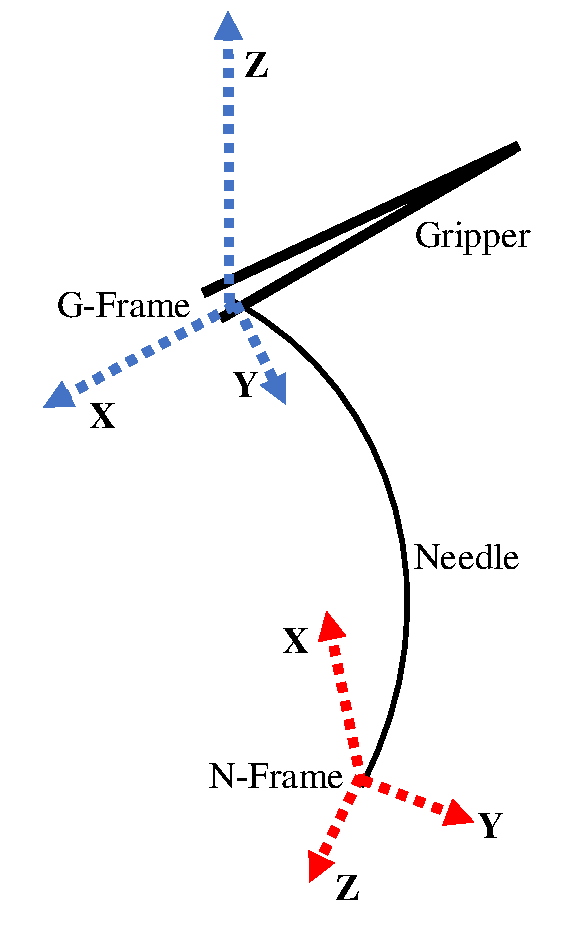
\includegraphics[scale=0.4]{figs/needle-frames.pdf}
    \caption{Gripper (G) and Needle (N) Frames of Reference (adapted from \cite[Figure 2(a)]{needle-grasp}). The G-Frame orients its origin at the tip of the gripper with Z-axis perpendicular to the gripper jaws; X-axis points parallel to the gripper, outwards. The N-Frame orients its origin at the needle tip, in this application needles are curved into a circular shape. The X-axis points towards the centre of needle curvature; Z-axis points tangent to the needle curvature, outwards.}
    \label{fig:needle-frames}
\end{figure}
\par{Four degrees of freedom are given for needle grasp; $\omega_{1}$ is rotation around the G-Frame Z-axis, $\omega_{2}$ is rotation around the G-Frame Y-axis, $\omega_{3}$ is rotation around an axis in the needle plane perpendicular with the X-axis in the N-Frame. Finally, $\vartheta_{0}$ is the insertion translation for the gripping point selected along the negative X-axis in the G-Frame. Following notation from the paper, $\varphi_0$ is the distance in insertion translation while $\varphi_1$, $\varphi_2$, $\varphi_3$ are respective rotation angles for $\omega_{1}$, $\omega_{2}$ and $\omega_{3}$.}

\par{Forward-kinematics are then derived, giving a translation matrix from the G-Frame to the N-Frame, denoted $g_{GN}$ and described by Equations \ref{eqn:matrix} \ref{eqn:R} and \ref{eqn:P} ($s_n$ denotes $\sin(\varphi_n)$; $c_n$ denotes $\cos(\varphi_n)$ and $r_n$ is the radius of needle curvature).}
\begin{equation}
    g_{GN}(\varphi) = 
      \begin{bmatrix}
      R(\varphi) & P(\varphi)\\
      0 & 1
      \end{bmatrix}
      \label{eqn:matrix}
\end{equation}
\begin{equation}
    R(\varphi) =  
    \begin{bmatrix}
    s_1 s_3 - c_1 c_3 s_2 & - c_1 c_2 & - c_3 s_1 - c_1 s_2 s_3 \\
    -c_1 s_3 - c_3 s_1 s_2 & - c_2 s_1 & c_1 c_3 - s_1 s_2 s_3 \\
    -c_2 c_3 & s_2 & -c_2 s_3
    \end{bmatrix}
    \label{eqn:R}
\end{equation}
\begin{equation}
    P(\varphi) = 
    \begin{bmatrix}
    r_n c_1 s_2 (c_3 - 1)-r_n s_1 s_3 - \varphi_0\\
    r_n c_1 s_3 + r_n s_1 s_2 (c_3 - 1)\\
    r_n c_2 (c_3 - 1)
    \end{bmatrix}
    \label{eqn:P}
\end{equation}

Needle grasp variants may be explored by changing parameters $\varphi_0$, $\varphi_1$, $\varphi_2$ and $\varphi_3$. As some configurations are invalid due to reach-ability, joint limits and/or link collision constraints, a feasibility algorithm is developed to assert invalid end-affector positions. Finally, a needle grasp selection algorithm is constructed~\cite[Algorithm 1]{needle-grasp}. This operates by taking a set input of potential needle grasps and for each grasp the feasibility over given needle suturing trajectory positions is computed. For needle grasps and trajectory positions deemed feasible, some performance metrics are computed for later comparison.

In experimentation, 3410 pre-set needle grasp positions are evaluated for two suturing trajectories (described as ``needle insertion'' and ``needle extraction''). Findings show that 7.1\% of grasps are feasible for needle insertion with 30.1\% feasible for extraction. Finally, an optimal grasping pose is shown which scores best on performance metrics for both trajectories. 

\subsection{Analysis - I}
This work details a process to compare or otherwise discount needle grasp poses for the suturing task. However, for full automation of suturing the question remains as to how these initial pose candidates are generated - no explanation is given for this. The authors mention that execution time for the 3410 poses used on a reasonably high end desktop machine is in the order of minutes. In a real world scenario the algorithm inputs would not be known before a surgery has begun - they would have to be computed ad-hoc. It is judged that minutes of processing time is too lengthy to expend during a surgical procedure. Thus, in its current form this is not usable in theatre. The authors suggest that this may be remedied by implementing the algorithm in faster code. As an alternative, the algorithm described could be used to label numerous grip poses with the evaluation metrics outlined in the paper. These data could then be used for supervised deep learning to train a machine capable of inferring an optimal needle grasp for any given scenario. This model could be more computationally efficient and adjusted for general use by tweaking the training data generated.    
\subsection{Literature - II}
Surgical procedures can regularly cause bleeding from severed tissue capillaries or internal veins/arteries. Deposited blood must be removed during surgery as to clear the view of the site, this is called hemostasis. \citeauthor{blood-suck} propose a solution to automate hemostasis for RMIS~\cite{blood-suck}. They detail an image processing technique to segment areas of blood identified in camera frames from the operating site. The processing method makes use of multiple temporal frames to identify moving blood pixels, a convolutional neural network is trained to achieve this. With blood location identified, a second algorithm computes the trajectory required for a suction device. These processes are tested on simulated blood flow scenes~\cite[Figure 4]{blood-suck}. In a usability test, the dVRK is used to upload software to a da Vinci machine equipped with camera and a suction tool. An artificial cavity is used with fake blood injected at different points. The system built is shown to consistently remove over 93\% of blood in less than a minute from reaction time through to trajectory completion. Authors note this as the first completely automated hemostasis, complete with dVRK integration. 

\subsection{Analysis - II}
The publication shows successful development of blood suction automation and a realistic test with a da Vinci machine. However, the computer vision method used necessitates use of multiple frames for detecting moving blood only. This could cause limitations of the system, in particular very slow or stationary blood pools may not be detectable with this method. In addition, no test is given where the camera is shaken or otherwise moved as would likely occur in a real surgical procedure, this could cause erroneous segmentation. Per-image segmentation techniques have become highly accurate in recent years. For example Mask R-CNN, developed by Facebook, is shown to score high accuracy on the MS COCO challenge\footnote{MS COCO: Microsoft's Common Objects in Context, online: \url{https://cocodataset.org/} - Accessed 15\textsuperscript{th} March 2022}~\cite{mask-rcnn}. In future research, a per-image segmentation method may yield resilience to camera tremors and/or highly correlated temporal frames. 

%In addition, automation of such tasks is thought to give rise to a new method for training robot operators. Work by 

\section{Conclusions}
This essay has investigated software and hardware innovations in RMIS looking specifically at those compatible with the dVRK. For the tooling innovations discussed, it is judged that further evaluation work will better illustrate performance of both devices. For the automation methods, a suggestion is given that the gripper pose selection algorithm could be used as a data labelling mechanism for training a more general AI solution. A suggested variation of the computer vision pipeline for automated hemostasis is also given. Finally, this report complements functionality of the dVRK, enabling all research discussed.
\printbibliography

\end{document}